\chapter[Marco Teórico]{Marco Teórico}
\label{chap:marco}
\section{La evolución del universo}
\label{sec:universo}
El universo tal y como lo conocemos hoy está poblado de cuerpos colosales, sorprendentes e incluso hermosos. Las estrellas, las nébulas y las galaxias son formaciones a las que estamos acostumbrados y que están presentes en donde quiera que nos adentremos en el cielo. Pero fue un proceso muy largo y turbulento para llegar a lo que hoy observamos y consideramos habitual, como nuestro sistema solar, un proceso que aún está lleno de incógnitas y de teorías que si bien se ajustan a las observaciones y predicciones, no están completamente comprobadas. La siguiente sección trata de resumir el conjunto de teorías y hechos que hacen parte de la visión más ampliamente aceptada como la historia del universo.


\subsection{El Principio cosmológico y el problema del Horizonte}
Las teorías que describen los momentos que precedieron al \textit{Big-Bang} y el análisis del fondo de radiación de microondas (CMB por sus siglas en inglés) han brindado un panorama de lo que que parece ser el inicio del universo y su progreso hasta lo que conocemos hoy en día; un universo que cumple con el principio cosmológico\cite{loeb}. Las fórmulas de la relatividad general de Einstein muestran cómo la estructura del Espacio-Tiempo se ve curvada por la presencia de la masa, pero al intentar aplicar estas fórmulas para mostrar la dinámica del universo, hay que considerar un modelo para éste. Dada la complejidad matemática que pueden llegar a tener estas fórmulas en el caso general, fue necesario considerar el caso más simple posible, dictado por el principio cosmológico. Bajo este principio, el universo es isotrópico y homogéneo, lo cual quiere decir que el universo tiene una distribución homogénea y esta distribución se cumple en cualquier dirección en la cual se observe. Se podría pensar que los planetas, estrellas, galaxias y otros cuerpos nombrados anteriormente, los cuales además de todo están separados por vastos vacíos casi absolutos, serían el perfecto contraejemplo para la suposición de Einstein, pero este enunciado hace referencias a escalas mucho mayores a las que podría abarcar cualquiera de estos cuerpos. Para dar una idea de la escala de distancias tratadas, la Vía Láctea tiene un tamaño aproximado de $30kpc$, pero si partimos el universo en cubos, por ejemplo de $90Mpc$, veremos que estos cubos comparten características casi idénticas, como por ejemplo, la densidad promedio, emisión de luz e incluso temperatura \cite{bang}. 

Este hecho antes de ser tranquilizante (vivimos en lo que sería el caso ideal de un universo), es bastante alarmante puesto que no puede ser coincidencia que lugares tan apartados del universo posean la misma temperatura, y no son dos lugares sino todos los rincones observados del universo los que cumplen con dicho principio. El problema radica en que la forma de comunicación más rápida existente entre dos cuerpos es la luz, y por ende la \textcolor{red}{comunicación} entre dos lugares del universo estará limitada por la distancia que los separa. De esta manera, si consideramos que el universo tiene una edad aproximada de $13.8Gyr$, no hay forma para que dos puntos opuestos (separados por $\approx 28Gly$) hayan tenido algún intercambio tal que les hubiese permitido estar en condiciones iguales hoy en día. 


\subsection{La Era Inflacionaria}
\label{sub:infl}
La teoría que hasta la fecha mejor resuelve esta incongruencia conocida como el \textit{Problema del Horizonte} es la teoría de la inflación. Ésta supone que en sus primeros instantes (al rededor de tiempos de $\sim 10^{-33} seg$), el universo pasó por un proceso de crecimiento acelerado, llegando incluso a velocidades superlumínicas. Existen varias versiones de esta época y no se ha logrado explicar a fondo la física detrás de este comportamiento. Entre las formas de explicarlo o describirlo, una explica que esta expansión se dio gracias a un estado que se conoce como \textit{falso vacío}, el cual no es mínimo estado de la densidad energética para un campo escalar, pero sí es un mínimo local, sólo que es inestable. En dicho estado se pudo dar una inflación de una sección tan pequeña que pudiese ser homogénea en sí, causando que el espacio resultante de la inflación replicara estas características. Dado el carácter atractivo (signo negativo) de la fuerza gravitacional es posible una expansión en donde se conserve la energía (Se ``crea'' energía al expandir que es compensada por la \textit{energía negativa} de la gravedad)\cite{bang}. 

\begin{figure}[H]
	\centering
	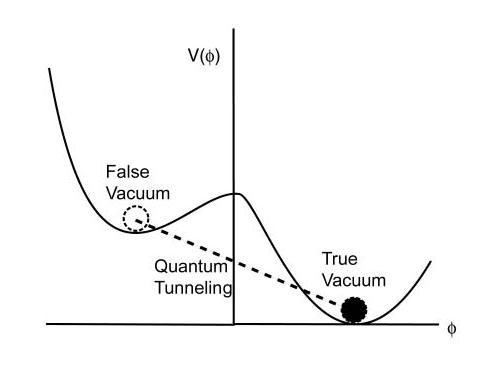
\includegraphics[width=8.5cm]{MarcoTeorico/figure7}
	\caption[Falso vacío y verdadero vacío ]{Falso vacío y verdadero vacío \footnotemark}
	\label{fig:falsevac}
\end{figure}
\footnotetext{Imagen tomada de \url{http://ned.ipac.caltech.edu/level5/Watson/Watson5_3.html}}

Otra forma de ver la inflación es pensando en que cualquier irregularidad presente en el universo cuando aún cabía en la palma de la mano se vería alisada por una expansión de dichas magnitudes. La difusión de los primeros fotones logró erradicar cualquier irregularidad en pequeña y gran escala de toda la materia ligada a la radiación electromagnética\cite{loeb}. En cualquiera de los casos, el resultado final de la inflación es un universo con las características que observamos en todas direcciones. 

Se cree que las galaxias y cuerpos que actualmente pueblan el universo se generaron a raíz  de las fluctuaciones cuánticas presentes en él cuando su tamaño fue lo suficientemente pequeño para que éstas tuvieran un efecto relevante en su estructura. En ese caso estas fluctuaciones de pequeña escala crecerían hasta tener un gran tamaño y se convertirían con el paso del tiempo en lo que hoy observamos como cuerpos estelares. Pero \textit{¿cómo es que estas fluctuaciones cuánticas siguieron presentes si la época inflacionaria borró cualquier irregularidad dando a un universo homogéneo?} La respuesta reside en cerca de un cuarto del contenido energético del universo: la materia oscura. 

\subsection{El equilibrio gravitacional y la composición del universo}
\label{sub:grav}
Observaciones y mediciones de los espectros de galaxias y estrellas lejanas no sólo nos brindan información de su composición, sino que también de su dinámica. Las alteraciones en el espectro pueden deberse a varios factores, en especial el corrimiento hacia el rojo, para el cual existen tres principales motivos. El primero es debido al Efecto Doppler, que al igual que con el sonido, la longitud de onda aumenta (se corre hacia el rojo) cuando el emisor y el observador se alejan a grandes velocidades; el segundo es dictado por la relatividad general, cuando una onda electromagnética está escapando de un campo gravitacional; y el tercero, de mayor interés para efectos de la discusión a seguir, es el corrimiento al rojo (o \textit{redshift}) intrínseco debido a la expansión del universo. 

Observaciones de diferentes espectros atómicos en el universo han mostrado que incluso corrigiendo los corrimientos dados por movimientos relativos y por campos gravitacionales, siempre hay un corrimiento al rojo remanente. Un fotón emitido en un dicho momento tendrá una longitud de onda definida, pero si el universo se expande (el espacio donde se desplaza se expande), al cabo de un tiempo este fotón tendrá una longitud de onda menor que la que tenía inicialmente. De esta manera se ha observado que el universo se está expandiendo, y además es una herramienta de gran utilidad para definir distancias de objetos lejanos. Al observar objetos distantes, observamos su pasado, pues lo que nos llega es la luz emitida tiempo atrás, cuando el universo era un poco más pequeño, de manera que a mayor redshift en el espectro, más antiguo es el objeto que observamos.

Si consideramos que la densidad es constante en el universo, esto permite realizar un análisis local obviando el efecto del resto del universo dada la simetría esférica. La energía total por unidad de masa en una esfera de radio $r$ es una expresión dada por la suma de energía cinética, por el movimiento de las partículas, y la energía gravitacional potencial existente entre estas, así, $E=\frac{1}{2}v^2-\frac{GM}{r}$, en donde $G$ es la constante gravitacional y M estará dada considerando una densidad $\rho$ uniforme en el volumen de la esfera. Reorganizando los términos, se puede llegar a la Ecuación (\ref{eq:En}), en donde $\Omega=\frac{\rho}{\rho_c}$ y el término $\rho_c$ se conoce como la densidad crítica.

\begin{equation}
E=\frac{1}{2}v^2(1-\Omega)\\
\label{eq:En}
\end{equation}

Si la densidad promedio de materia en el universo $\rho$ es menor que la densidad crítica $\rho_c$  entonces tendremos que $E<0$ lo cual significa que la gravedad nunca podrá contrarrestar la expansión actual y toda galaxia está condenada a una muerte solitaria pues esta expansión continuará indefinidamente. Esto se conoce como la solución de un universo abierto. En cambio, si la densidad está por encima de la densidad crítica se tiene que la expansión se detendrá en un punto y comenzará a revertirse debido a la atracción gravitacional terminando en lo que se ha acuñado como el \textit{Big-Crunch}. Esta segunda solución se conoce como el universo cerrado. Finalmente, la tercera solución corresponde al universo plano en la que $E=0$ y la densidad de materia es exactamente igual a la densidad crítica. Esta tercera es la que se ha observado que coincide con la realidad, pero este es un equilibrio críticamente inestable, ya que por más homogéneo que se considere el universo, cualquier fluctuación crecerá con el paso del tiempo. Así si una pequeña sección supera la densidad crítica, comenzará a ejercer una mayor fuerza que el resto del universo, absorbiendo materia de las partes en donde la densidad es menor a la crítica. Rápidamente la parte densa se volverá más y más densa, contrario a lo que sucede con las secciones menos densas; una vez roto el equilibrio no hay vuelta atrás.

Como se dijo en la Sección \ref{sub:infl}, la inflación eliminó cualquier fluctuación de materia interactuante con la radiación, de manera que se estableció un equilibrio irrompible, en donde la formación de estrellas y galaxias se vuelve imposible. La materia oscura es la teoría de mayor acogida y validez para romper no sólo esta paradoja, sino que también otros fenómenos observados como las lentes gravitacionales y las velocidades de rotación de sistemas binarios. Para todos estos, se necesita que exista una cantidad de materia mayor que la observada; es decir, una cantidad mayor de materia que la que interactúa con la radiación electromagnética (materia ordinaria). De allí su nombre, la materia oscura es un tipo de materia con las mismas características gravitacionales que la materia ordinaria, pero no interactúa con ningún tipo de luz, de manera que no se puede observar de manera directa. La única forma de detectarla es por efectos indirectos, como la medición la cantidad de materia necesaria para que los fenómenos nombrados anteriormente tengan un sentido físico. 

Volviendo al universo primitivo, las fluctuaciones cuánticas generaron cambios en todo tipo de materia, pero la inflación sólo afecto aquella materia interactuante con la radiación, de manera que estas irregularidades quedaron grabadas en la materia oscura y crecieron junto con todo el universo. Esto creó regiones con mayor atracción gravitacional, causando que la materia ordinaria cayera en dichas zonas, juntándose, creciendo y formando cuerpos celestes. De manera que (bajo este punto de vista) es gracias a la presencia de la materia oscura que se pudo dar un universo tal y como lo conocemos, y es más, simulaciones de muy alto nivel de cuerpos de materia oscura, en comparación con las imágenes de estructura a gran escala del universo, muestran que la materia ordinaria se organiza exactamente en donde se generan mayores concentraciones de materia oscura, por el efecto nombrado anteriormente. Mediciones de la distribución de materia muestran que la materia oscura suma aproximadamente un $25\%$ de la energía total del universo, mientras que la materia ordinaria forma alrededor de un $5\%$. 

Estos porcentajes se conocen por mediciones y estimaciones, e incluyéndolos en la Ecuación (\ref{eq:En}), puesto que según las observaciones el universo debería ser plano y $\rho\approx\rho_c$. Al sumar toda la densidad de materia oscura y materia ordinaria, aún faltaría un gran porcentaje de densidad energética para cumplir la condición nombrada arriba, de manera que se plantea la energía oscura para cumplir con esa cuota. Es muy poco lo que se sabe acerca de la energía oscura y son muchas las teorías y vertientes entorno a ella, desde la energía de polarización de vacío hasta un fluido que llena todo el espacio tiempo. Entre las cosas que se pueden afirmar de ésta es que es cerca del $70\%$ del contenido energético del universo y es la responsable de la expansión de este (contrarrestada únicamente por la materia que conforma el otro $30\%$).

\subsection{Variables Relevantes y Parametrizaciones} 
Una vez explicada la historia que conllevó a la evolución del universo, es importante rescatar las parametrizaciones de cada fenómeno nombrado anteriormente, puesto que estas variables son los parámetros de ingreso a las simulaciones que se realizaron. Empezando por la expansión del universo, esta se mide por un factor de escala $a(t)$ que varía con el tiempo, tiene un valor de $1$ en la actualidad y para su definición se dice que si una distancia tiene una longitud $r(t_1)$ en dicho tiempo, entonces en $t_2$ estará definido por,

\begin{equation}
r(t_2)=r(t_1)\left[\frac{a(t_2)}{a(t_1)}\right]
\label{eq:at}
\end{equation}

Este factor es el que permite llevar cuenta de la expansión del universo a lo largo de una simulación, y puede definirse a partir del \textit{redshift} $z$, $a(t)=\frac{1}{1+z(t)}$ del cual se hablaba en la Sección \ref{sub:grav}. En la Figura \ref{fig:red} se observa un diagrama que muestra la historia del universo desde el Big-Bang, en la parte más externa cuando $z$ tiende a infinito, hasta la actualidad en el centro, donde $z=0$. Bajo este parámetro se fijan los tiempos de simulación y los intervalos de generación de \textit{snapshots} para las simulaciones realizadas. Asimismo, debemos incluir la versión matemática de la ley de expansión de Hubble, en donde se establece (a partir de observaciones) que la velocidad relativa (y por ende el corrimiento al rojo) de un objeto distante será proporcional a su distancia, donde $H_0$ es conocida como la constante de Hubble,

\begin{equation}
v=H_0r
\label{eq:hub}
\end{equation}

\begin{figure}[H]
	\centering
	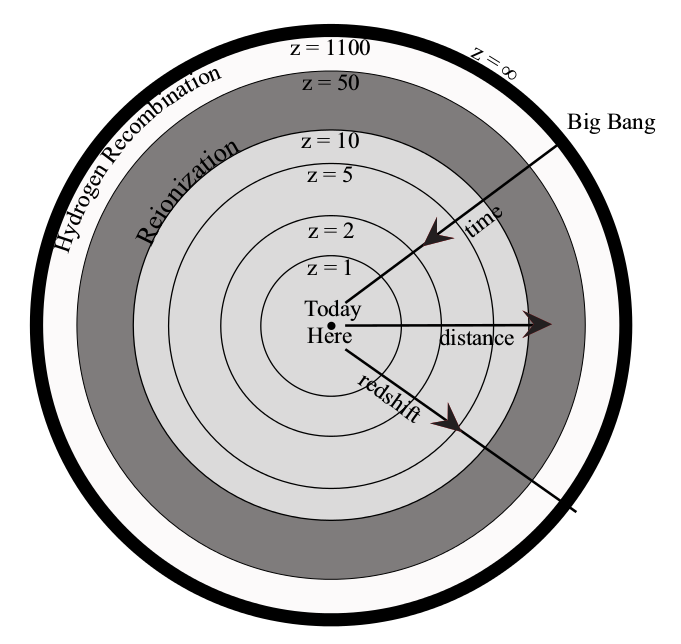
\includegraphics[width=9cm]{MarcoTeorico/historia}
	\caption[Diagrama de tiempo del universo]{Diagrama de tiempo del universo\footnotemark}
	\label{fig:red}
\end{figure}
\footnotetext{Imagen tomada de \cite{loeb}}

Pero la constante de Hubble puede cambiar con el avance del tiempo, de manera que como las demás constantes se define un valor actual y su avance hacia atrás en el tiempo. Por ejemplo, volviendo a la ecuación \ref{eq:En}, se asume que en el presente $\Omega_0=1=(\Omega_\Lambda+\Omega_m+\Omega_r)$, para lo cual la primera contribución corresponde a la densidad de energía del vacío (Energía Oscura), el segundo término corresponde a la materia (tanto oscura como ordinaria o bariónica ($\Omega_b$) y la contribución energética de la radiación. Estos parámetros de distribución de energía son las semillas que pueden llevar a diferentes universos y son precisamente los parámetros de entrada para las simulaciones realizadas en este proyecto. La expresión general para los parámetros está dada por la Ecuación (\ref{eq:total}).

\begin{equation}
\frac{H(t)}{H_0}=\left[\frac{\Omega_m}{a^3}+\Omega_\Lambda+\frac{\Omega_r}{a^4}\right]^{\frac{1}{2}}
\label{eq:total}
\end{equation}


\section{Simulación en Paralelo y Análisis}
Como se dijo en la Sección \ref{sec:universo}, la materia oscura tiene las mismas propiedades gravitatorias que la materia ordinaria u observable, pero la supera en cantidad por casi 5 veces en todo el universo. Es por esto que para analizar las estructuras a gran escala el universo, la distribución de materia, los grandes halos y la dinámica de la materia en el universo se puede partir del análisis de materia oscura, puesto que se espera que la materia ordinaria esté ubicada en donde existan mayores concentraciones de materia oscura. Si bien no tenemos forma de observar los cambios en el universo si se cambia la distribución de energías, se pueden realizar simulaciones a gran escala de todo el universo variando los parámetros cosmológicos. En la siguiente sección se explicará brevemente las características de los algoritmos utilizados y su modo de funcionamiento.


\subsection{Gadget-2 y N-GenIC}

Toda simulación de un entorno estará limitada por el recursos computacionales que se tengan, como por ejemplo el tiempo de simulación, la cantidad de procesadores disponibles y la cantidad de memoria que se puede ocupar. De manera que la eficiencia de un código estará dictada por la eficiencia en consumo de dichos recursos; qué tantos recursos consume y qué tan exactos son los resultados obtenidos. Existe una gran variedad de códigos para la simulación de $N$ partículas con diversas ventajas y desventajas entre cada uno, pero la principal diferencia radica en el método de análisis de cada código para realizar aproximaciones a pequeña y gran escala, permitiendo así una cierta tolerancia sin comprometer mayor cantidad de recursos. Gadget-2 es un código creado por Volker Springel y publicado en el 2005\cite{gadget} para realizar grandes simulaciones cosmológicas de $N$ cuerpos. 


